\documentclass[a4paper,11pt]{article}

\usepackage{wrapfig}
\usepackage{amsmath}
\usepackage{pgfplots}
\usepackage{xcolor}
\usepackage[most]{tcolorbox}
%Russian-specific packages
%--------------------------------------
\usepackage[T2A]{fontenc}
\usepackage[utf8]{inputenc}
\usepackage[russian, english]{babel}
%--------------------------------------

\graphicspath{ {./img/} }

\definecolor{lemonchiffon}{rgb}{1.0, 0.98, 0.8}
\newtcolorbox{mainblock}{colback=lemonchiffon,grow to right by=-10mm,grow to left by=-10mm,
boxrule=0pt,boxsep=0pt,breakable} % настройки области с изменённым фоном
\definecolor{block-gray}{gray}{0.95} % уровень прозрачности (1 - максимум)
\newtcolorbox{importantblock}{colback=block-gray,grow to right by=-10mm,grow to left by=-10mm,
boxrule=0pt,boxsep=0pt,breakable} % настройки области с изменённым фоном

\makeatletter
\newcommand{\settag}[1]{
  \tag*{(#1)\qquad}
  \edef\@currentlabel{\theequation#1}}
\makeatother

\title{26. Методы Рунге-Кутты. Подпрограмма \textbf{RKF45}}
\author{Андрей Бареков \and Ярослав Пылаев \and По лекциям Устинова С.М.}
\date{\today}

\begin{document}
\maketitle
\newpage

\noindent Недостатком методов Адамса является то, что они не самостартующие, и их разностные уравнения имеют порядок выше первого.
  От этого недостатка свободны методы Рунге-Кутты.

\section{Методы Рунге-Кутты}
Разностные уравнения этих методов имеют первый порядок\footnotemark, и степень точности повышается за счет увеличения объёма работы на каждом шаге.
\footnotetext{Одношаговые методы, one-step methods}
\begin{gather}
  \frac{dx}{dt} = f(t, x),\, x(t_0) = x_0 \\
  x_{n+1} = x_n + \int_{t_n}^{t_{n+1}} f(\tau, x(\tau))\,d\tau
\end{gather}
Воспользуемся формулой средних прямоугольников: \\
\marginpar {
  \footnotesize (*) явный метод ломаных Эйлера
}
\begin{equation}
  \begin{cases}
    x_{n+\frac{1}{2}}^* = x_n + \frac{h}{2} f(t_n, x_n)^{(*)} \\
    x_{n+1} = x_n + hf(t_n + \frac{h}{2}, x_{n+\frac{1}{2}}^*)
  \end{cases}
  \label{eq:HM}
\end{equation}
\begin{center}
  \small{Модифицированный метод ломаных Эйлера или метод Гойна}
\end{center}
Воспользуемся неявным методом трапеций:
\begin{equation}
  \begin{cases}
    x_{n+1}^* = x_n + hf(t_n, x_n)^{(*)} \\
    x_{n+1} = x_n + \frac{h}{2}(f(t_n, x_n) + f(t_{n+1}, x_{n+1}^*))
  \end{cases}
  \label{eq:ECM}
\end{equation}
\begin{center}
  \small{Метод Эйлера-Коши}
\end{center}
Оба метода имеют вторую степень точности, но функцию в этих методах мы вычисляем не один, а два раза. \\
\begin{importantblock}
  Эту идею можно обобщить в следующем виде:
  \begin{equation}
    \begin{cases}
      k_1 = hf(t_n, x_n) \\
      k_2 = hf(t_n + \alpha h, x_n + \beta k_1) \\
      x_{n+1} = x_n + p_1k_1 + p_2k_2
    \end{cases},
    \label{eq:RKM}
  \end{equation}
  Параметры $\alpha,\, \beta,\, p_1,\, p_2$ выбираются так, чтобы получить наибольшую степень точности.
\end{importantblock}
\begin{align*}
  F(u(h), v(h)) &= F(u(0), v(0)) \\
                &+ \frac{h}{1!} \frac{dF}{dh}(u(0), v(0)) \\
                &+ \frac{h^2}{2!} \frac{d^2F}{dh^2}(u(0), v(0)) \\
                &+ \dots
\end{align*}
\[\frac{dF}{dh} = \frac{\partial F}{\partial u} \times \frac{du}{dh} + \frac{\partial F}{\partial v} \times \frac{dv}{dh}\]
\marginpar {
  \footnotesize $x^{'}(t) = f(t, x)$
}
\begin{equation}
  \begin{aligned}
    x_{n+1} &= x_n + \frac{h}{1!}x^{'}(t_n) + \frac{h^2}{2!}x^{''}(t_n) + \dots \\
            &= x_n + hf(t_n, x_n) + \frac{h^2}{2!}\frac{df(t, x)}{dt}(t_n) + \dots \\
            &= x_n + hf(t_n, x_n) + \frac{h^2}{2!}\Big (\frac{\partial f}{\partial t} \times \underbrace{\frac{dt}{dt}}_{1} + \frac{\partial f}{\partial x} \times \underbrace{\frac{dx}{dt}}_{f}\Big ) \Big |_{t=t_n} + \dots
  \end{aligned}
  \label{eq:KAWO}
\end{equation}
Раскладываем в ряд формулу (\ref{eq:RKM}) и сравниваем коэффициенты с формулой (\ref{eq:KAWO}):
\begin{align*}
  x_{n+1} &= x_n + p_1hf(t_n, x_n) + p_2hf(t_n + \alpha h, x_n + \beta hf_n) \\
          &= x_n + p_1hf(t_n, x_n) + p_2h\Big(f(t_n, x_n) + \frac{h}{1!}\frac{df}{dh}(t_n) + \dots\Big) \\
          &= x_n + p_1hf_n + p_2h\Big(f_n + h\Big(\frac{\partial f}{\partial t}\alpha + \frac{\partial f}{\partial x}\beta f \Big)\Big |_{t=t_n} + \dots\Big)
\end{align*}
\begin{importantblock}
  \begin{equation*}
    \begin{cases}
      p_1 + p_2 = 1 \\
      p_2\alpha = \frac{1}{2} \\
      p_2\beta = \frac{1}{2}
    \end{cases}
  \end{equation*}
  Для второй степени точности получаем $3$ уравнения с $4$ неизвестными $\Rightarrow$ мы имеем бесконечное множество методов Рунге-Кутты второй степени точности. \\
  Например:
  \[p_1 = 0,\, p_2 = 1,\, \alpha = \beta = \frac{1}{2}\]
  \begin{center}
    \small{Модифицированный метод ломаных Эйлера}
  \end{center}
  \[p_1 = p_2 = \frac{1}{2},\, \alpha = \beta = 1\]
  \begin{center}
    \small{Метод Эйлера-Коши}
  \end{center}
\end{importantblock}

\noindent Эта идея может быть продолжена для построения методов семейства Рунге-Кутты более высокой степени точности:
\begin{gather*}
  k_1 = hf(t_n,x_n), \, \dots, \, k_r = hf \bigg( t_n + \alpha_rh, \, x_n + \sum_{i=1}^{r-1}\beta_{ri}k_i \bigg), \, r=1,2,\dots,s, \\
  \boxed{x_{n+1} = x_n + \sum_{r=1}^s p_rk_r}
\end{gather*}
Наибольшую популярность получил метод Рунге-Кутты \textit{четвертой степени} точности:
\begin{equation}
  \begin{cases}
    k_1 = hf(t_n, x_n) \\
    k_2 = hf(t_n + \frac{h}{2}, x_n + \frac{1}{2}k_1) \\
    k_3 = hf(t_n + \frac{h}{2}, x_n + \frac{1}{2}k_2) \\
    k_4 = hf(t_n + h, x_n + k_3) \\
    x_{n+1} = x_n + \frac{1}{6}(k_1 + 2k_2 + 2k_3 + k_4)
  \end{cases}
  \label{eq:RKM4}
\end{equation}

\vspace{3mm}
\noindent Геометрическая интерпретация:
\begin{center}
  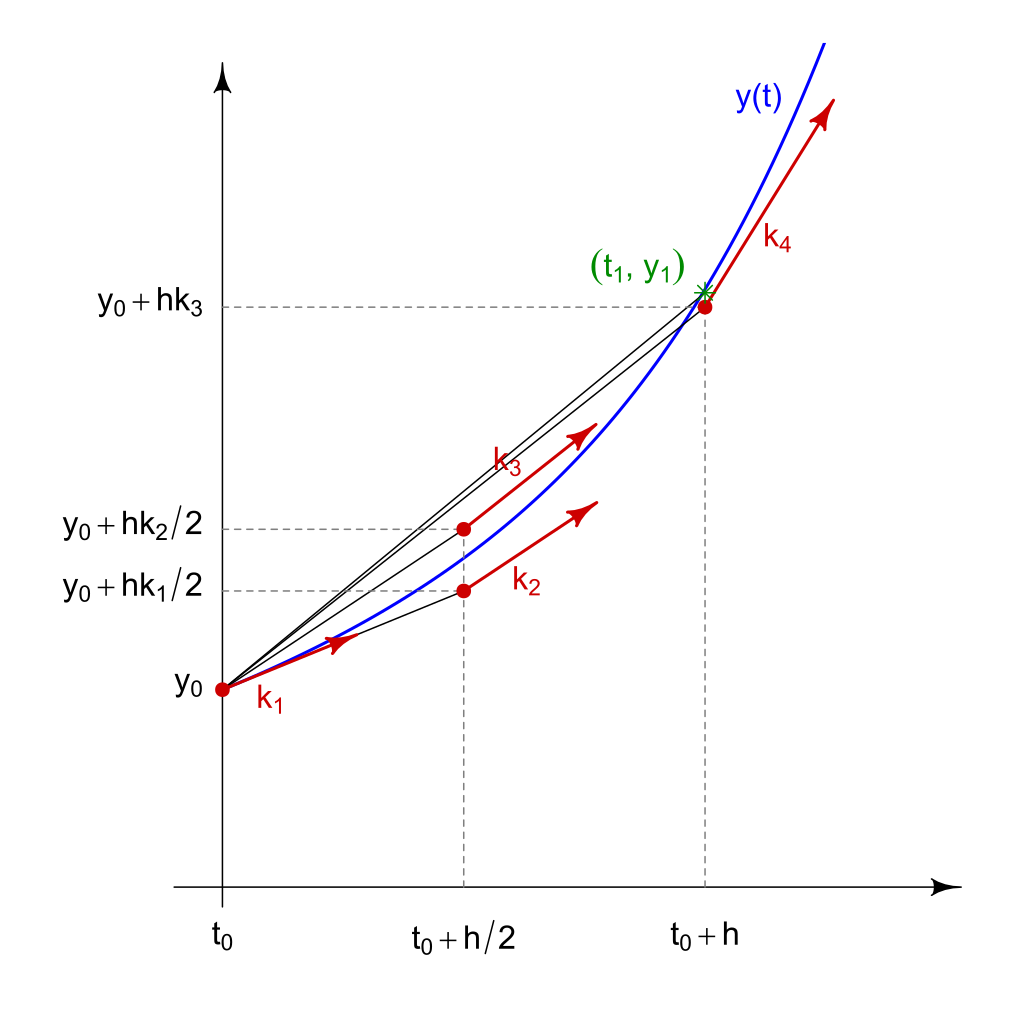
\includegraphics[scale=0.3]{img2.png} \\
  \small
  Именна параметров на изображении можно заменить в соотсветствии с используемыми в формулах нашего вида.
\end{center}

\noindent Рассмотрим частный случай:
\begin{gather*}
  f(t, x) = f(t),\quad k_2 = k_3 \\
  x_{n+1} = x_n + \frac{h}{6}(f(t_n) + 4f(t_n+\frac{h}{2}) + f(t_n + h))
\end{gather*}
Всё превратилось в квадратурную формулу Симпсона.

\section{Программа RKF45}
Программа построена на методах Рунге-Кутты четвертой и пятой степеней, при этом для получения решения по обоим методам используются одни и те же $k_i$. \\
\begin{align*}
  x_{n+1}^{(IV)} &= x_n + \sum_{i=1}^6 p_i k_i ^[\footnotemark^] \\
  x_{n+1}^{(V)}  &= x_n + \sum_{i=1}^6 p_i^* k_i
\end{align*}
\footnotetext{здесь $p_5$ и $p_6 = 0$}

\noindent Программа реализует переменный шаг интегрирования. Локальная погрешность оценивается по разности двух решений:
\[x_{n+1}^{(V)} - x_{n+1}^{(IV)} = \sum_{i=1}^6 (p_i^* - p_i)k_i\]
Если погрешность оказалась больше требуемой величины, то шаг уменьшается, а если меньше, то следующий шаг увеличивается.\footnotemark
\footnotetext{погрешность IV метода $\sim h^5$. Например, если погрешность в $29$ раз больше требуемой, шаг уменьшается в $2$ раза}
\[\textbf{RKF45}(\underbrace{N}_{\text{порядок системы}},\, X,\, T,\, TOUT,\, \underbrace{EA,\, ER}_{\text{погрешности}},\, \dots)\]
На входе в векторе $X$ размещается решение в точке $T$. На выходе в этом же векторе размещается решение в точке $TOUT$. Если интегрирование прошло успешно,
  то $T == TOUT$. \\
  $HPRINT$ - шаг визуализвции решения/шаг печати \\
  $TOUT = TOUT + HPRINT$

\end{document}
